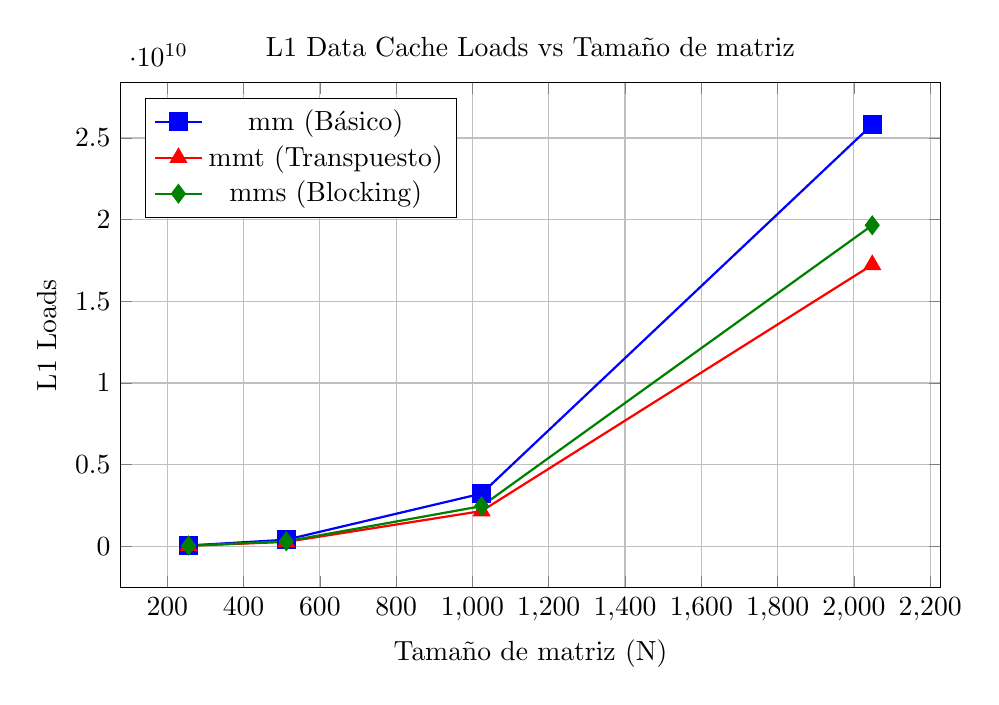
\begin{tikzpicture}
    \begin{axis}[
        title={L1 Data Cache Loads vs Tamaño de matriz},
        xlabel={Tamaño de matriz (N)},
        ylabel={L1 Loads},
        legend pos=north west,
        grid=major,
        width=12cm,
        height=8cm,
    ]
        \addplot[
            color=blue,
            mark=square*,
            thick,
            mark size=3pt,
        ]
        coordinates {
            (256, 51004911)
            (512, 404778774)
            (1024, 3230276569)
            (2048, 25823162241)
        };
        \addlegendentry{mm (Básico)}
        \addplot[
            color=red,
            mark=triangle*,
            thick,
            mark size=3pt,
        ]
        coordinates {
            (256, 34548801)
            (512, 271786720)
            (1024, 2160651349)
            (2048, 17237617045)
        };
        \addlegendentry{mmt (Transpuesto)}
        \addplot[
            color=green!50!black,
            mark=diamond*,
            thick,
            mark size=3pt,
        ]
        coordinates {
            (256, 38928205)
            (512, 308486652)
            (1024, 2460731377)
            (2048, 19660907418)
        };
        \addlegendentry{mms (Blocking)}
    \end{axis}
\end{tikzpicture}
